\documentclass{article}
\usepackage[T1,T2A]{fontenc}
\usepackage[utf8]{inputenc}
\usepackage[english,russian]{babel}
\usepackage{amsmath}
\usepackage{amsfonts}
\usepackage{amssymb}
\usepackage{makeidx}
\usepackage{listings}
\usepackage{setspace,amsmath}
\usepackage{graphicx}%Вставка картинок правильная
\usepackage{float}%"Плавающие" картинки
\usepackage{wrapfig}
\usepackage{comment}
\usepackage[document]{ragged2e}
\usepackage[export]{adjustbox}
\usepackage{subcaption}

\begin{document}

\begin{titlepage}
	\newpage
	
	\begin{center}
		\textbf{Федеральное государственное бюджетное образовательное учреждение высшего образования «Московский государственный университет имени М. В. Ломоносова»}\\
	\end{center}
	
	\vspace{8em}
	
	\begin{center}
		\Large Кафедра вычислительной механики \\ 
	\end{center}
	
	\vspace{2em}
	
	\begin{center}
		\Large \textsc{\textbf{Отчёт по задаче на работу с изображениями по теме:}}
		\\
		\Large \textsc{\textbf{ Фрактальное сжатие изображений \linebreak}}
	\end{center}
	
	\vspace{15em}
	
	
	
	\begin{flushright}
		\small
		\textbf{Преподаватель: Почеревин Роман Владимирович}\\
		\textbf{Студент 223 группы: Скворцов Андрей Сергеевич}\\
	\end{flushright}
	
	
	\vspace{\fill}
	
	\begin{center}
		Москва \\2024
	\end{center}
	
\end{titlepage}

\begin{center}

{\large\bf Отчёт по работе с BMP-изображениями в Python-3}

\end{center}

\textit{З\,а\,д\,а\,н\,и\,е.} Реализовать алгоритмы фрактального сжатия и восстановления изображения.

 
\textit{Р\,е\,ш\,е\,н\,и\,е.}  Используя библиотеки numpy и scipy, можно решить эту задачу проще. Кроме того используем библиотеки multiprocessing для распараллеливания программы:

\section{Загрузка изображений}

\begin{lstlisting}[language=Python]
import matplotlib.pyplot as plt
import matplotlib.image as mpimg
from scipy import ndimage
import numpy as np
from PIL import Image
import multiprocessing as mp
import datetime
\end{lstlisting}

\vspace{1em}

Пусть изображения заданы внутри программы. Выгрузим его как черно-белое при помощи функции get\_greyscale\_image(img):
\begin{lstlisting}[language=Python]

def get_greyscale_image(img):
	return np.mean(img[:,:,:2], 2)
\end{lstlisting}
Далее разобьем изображение на нужные нам блоки размера 4 на 4 вместо 8 на 8 при помощи функции reduce(img, factor):
\begin{lstlisting}[language=Python]
def reduce(img, factor):
	result = np.zeros((img.shape[0] // factor, img.shape[1] // factor))
	for i in range(result.shape[0]):
		for j in range(result.shape[1]):
			result[i, j] = np.mean(img[i * factor:(i + 1) * factor,
			j * factor:(j + 1) * factor])

	return result
\end{lstlisting}
\vspace{1em}

\section{Алгоритм фрактального сжатия}

\subsection{Генерация преобразованных блоков}

Теперь рассмотрим сам алгоритм фрактального сжатия изображения. Оно происходит при вызове функции compress. Сначала мы генерируем всевозможные блоки, которые мы можем получить при помощи нашего отображения, при помощи
функции generate\_all\_transformed\_blocks:
 
\begin{lstlisting}[language=Python]
def generate_all_transformed_blocks(img, source_size_block, 
destination_size_block, step):
	factor = source_size_block // destination_size_block
	transformed\_blocks = []
	for k in range((img.shape[0] - source_size_block) // step + 1):
		for l in range((img.shape[1] - source_size_block) // step + 1):
			S = reduce(img[k * step:k * step + source_size_block,
			l * step:l * step + source_size_block], factor)
			for direction, angle in candidates:
				transformed_blocks.append((k, l, direction, 
				angle, apply_transformation(S, direction, angle)))

	return transformed_blocks
\end{lstlisting}
\vspace{1em}

В этой функции мы исползуем функции поворота на угол кратный пи / 2 и отзеркаливание блока с последующим примением трансформации:

\begin{lstlisting}[language=Python]
def rotate(img, angle):
	return ndimage.rotate(img, angle, reshape = False)

def flip(img, direction):
	return img[::direction,:]

def apply_transformation(img, direction, angle, contrast = 1.0, 
brightness = 0.0):
	return contrast * rotate(flip(img, direction), angle) + brightness
\end{lstlisting}
\vspace{1em}

\subsection{Сжатие}

Далее для каждого блока размером 8 на 8 ищем наиболее похожий на него блок размера 4 на 4 и сохраняем параметры преобразования этого блока, а также координаты исходного блока:

\begin{lstlisting}[language=Python]
def compress(img, source_size_block, destination_size_block, step):
	transformations = []
	transformed_blocks = generate_all_transformed_blocks(img, 
	source_size_block, destination_size_block, step)
	
	i_count = img.shape[0] // destination_size_block
	j_count = img.shape[1] // destination_size_block
	for i in range(i_count):
		transformations.append([])
		for j in range(j_count):
			transformations[i].append(None)
			min_d = float('inf')
			D = img[i * destination_size_block:
			(i + 1) * destination_size_block, 
			j * destination_size_block:
			(j + 1) * destination_size_block]
			
			for k, l, direction, angle, S in transformed_blocks:
				contrast, brightness = 
				find_contrast_and_brightness2(D, S)
				
				S = contrast * S + brightness
				d = np.sum(np.square(D - S))
				if d < min_d:
					min_d = d
					transformations[i][j] = (k, l, direction, 
					angle, contrast, brightness)
					
					transformations_no_fratal[i][j] = S

	np.save('save_data_{}'.format(number), transformations_no_fratal)
	np.save('save_data_fractal_{}'.format(number), transformations)

	return transformations
\end{lstlisting}
\vspace{1em}

Для наибольшей схожести блоков подбираем яркость и контрастность при помощи функции find\_contrast\_and\_brightness2, причем схожесть определяется методом наименьших квадратов, реализованным в библиотеке numpy:
\begin{lstlisting}[language=Python]
def find_contrast_and_brightness2(D, S):
	A = np.concatenate((np.ones((S.size, 1)), 
	np.reshape(S, (S.size, 1))), axis = 1)
	
	b = np.reshape(D, (D.size,))
	x, _, _, _ = np.linalg.lstsq(A, b, rcond=None)

	return x[1], x[0]
\end{lstlisting}

\vspace{1em}

\subsection{Восстановление изображения после фрактального сжатия}

Теперь рассмотрим алгоритм восстановления описанный в функции decompress. Самое полезное для нас в сжимающем отображении это наличие неподвижных точек в каждом блоке, поэтому для восстановления изображения 
нужно просто применить это отображение несколько раз к случайному изображению:

\begin{lstlisting}[language=Python]
def decompress(transformations, source_size_block, 
destination_size_block, step, nb_iter):

	factor = source_size_block // destination_size_block
	height = len(transformations) * destination_size_block
	width = len(transformations[0]) * destination_size_block
	iterations = [np.random.randint(0, 256, (height, width))]
	cur_img = np.zeros((height, width))
	for i_iter in range(nb_iter):
		for i in range(len(transformations)):
			for j in range(len(transformations[i])):
				k, l, flip, angle, 
				contrast, brightness = transformations[i][j]
				
				k = int(k)
				l = int(l)
				flip = int(flip)
				S = reduce(iterations[-1][k * step:
				k * step + source_size_block,l * step:
				l * step + source_size_block], factor)
				
				D = apply_transformation(S, flip, angle, 
				contrast, brightness)
				
				cur_img[i * destination_size_block:
				(i + 1) * destination_size_block,
				j * destination_size_block:
				(j + 1) * destination_size_block] = D
				
		iterations.append(cur_img)
		cur_img = np.zeros((height, width))

	return iterations
\end{lstlisting}
\vspace{1em}

Сохраним изображение:
\vspace{1em}

\begin{lstlisting}[language=Python]
	plt.imsave('result_{}.bmp'.format(number1), 
	iterations[nb_iter - 1], cmap='gray')
\end{lstlisting}
\vspace{1em}
\subsection{Восстановление размеров изображения}

После восстановления изображения мы получили его уменьшенную версию, по сравнению с исходным вариантом. Масштабируем его при помощи функции scale\_image:

\begin{lstlisting}[language=Python]
def scale_image(input_file, output_file, scale):
	try:
		img = Image.open(input_file)
		width, height = img.size
		new_width = width * scale
		new_height = height * scale
		new_img = Image.new('RGB',(new_width, new_height))

		for k in range(new_width):
			for l in range(new_height):
				i = k // scale
				j = l // scale
				pixel_sum = [0,0,0]
				for x in range(2):
					for y in range(2):
						if i + x < width and j + y < height:
						  pixel = img.getpixel
						  ((i + x, j + y))
							
						  pixel_sum[0] += pixel[0]
						  pixel_sum[1] += pixel[1]
						  pixel_sum[2] += pixel[2]
				pixel_avg=(pixel_sum[0] // 4, pixel_sum[1] // 4, 
				pixel_sum[2] // 4)
				
				new_img.putpixel((k, l), pixel_avg)
				new_img.save(output_file)
	except Exception as e:
		print(f"An error occurred: {e}")
\end{lstlisting}
\vspace{1em}

\section{Дополнительный способ сжатия}

Помимо метода фрактального сжатия я рассмотрел вариант сохранения наиболее похожих блоков, для уменьшения потери качества изображения. Он реализуется вместе с методом фрактального сжатия и, в некотором смысле, идет параллельно ему.

Алгоритм восстановления прост: считывается NDarray и преобразуется в изображение

\begin{lstlisting}[language=Python]
def decompress_ultra_mega_sposob(transformations, 
source_size_block, destination_size_block):

	height = len(transformations) * destination_size_block
	width = len(transformations[0]) * destination_size_block
	cur_img = np.zeros((height, width))

	for i in range(len(transformations)):
		for j in range(len(transformations[i])):
			cur_img[i * destination_size_block:
			(i + 1) * destination_size_block,
			j * destination_size_block:
			(j + 1) * destination_size_block] = transformations[i][j]

	return cur_img
\end{lstlisting}
\vspace{1em}

\section{Анализ подбора коэффициентов сжатия}

Для меньшей потери качества было проведено исследрование на коэффициенты сжатия: какого размера брать ранговые и доменные блоки.

Я рассматривал сжатия 4 в 2, 6 в 3, 8 в 4 и 10 в 5 и получил следующие результаты(в данном лучае сжатие k в l означает, что мы превращаем блоки k * k в блоки l * l):

\begin{figure}[h]
	\subcaptionbox{Исходная маленькая картинка}{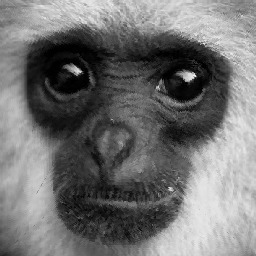
\includegraphics[width=0.3\textwidth]{input_1.jpg}}\hfill
	\subcaptionbox{Исходная большая картинка}{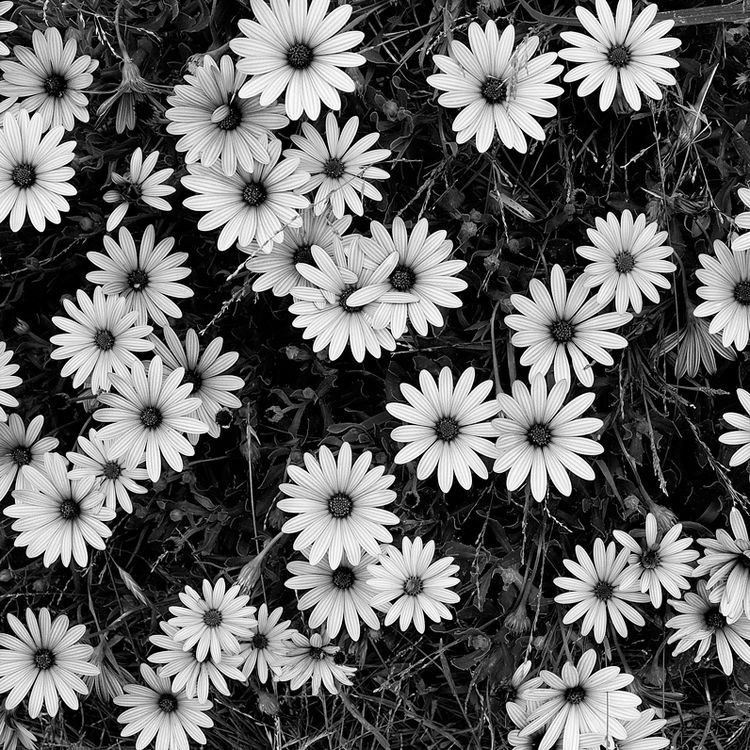
\includegraphics[width=0.3\textwidth]{input_2.jpg}}
\end{figure}

\subsection{Малое изображение}


\begin{figure}[h]
	\subcaptionbox{Фрактальное сжатие 4 в 2}{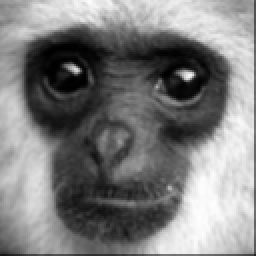
\includegraphics[width=0.2\textwidth]{result_1.jpg}}\hfill
	\subcaptionbox{Способ сохранения 4 в 2}{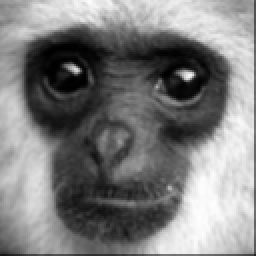
\includegraphics[width=0.2\textwidth]{result_ultra_mega_sposob_1.jpg}}\hfill
	\subcaptionbox{Фрактальное сжатие 6 в 3}{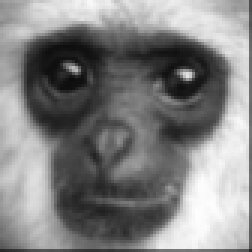
\includegraphics[width=0.2\textwidth]{result_11.jpg}}\hfill
	\subcaptionbox{Способ сохранения 6 в 3}{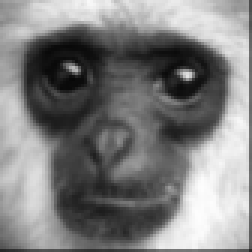
\includegraphics[width=0.2\textwidth]{result_ultra_mega_sposob_11.jpg}}
\end{figure}


\begin{figure}[h]
	\subcaptionbox{Фрактальное сжатие 8 в 4}{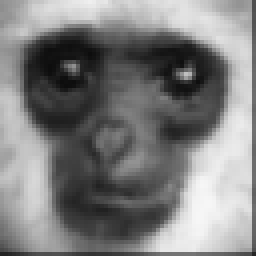
\includegraphics[width=0.2\textwidth]{result_12.jpg}}\hfill
	\subcaptionbox{Способ сохранения 8 в 4}{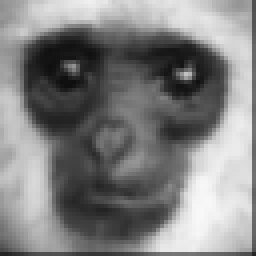
\includegraphics[width=0.2\textwidth]{result_ultra_mega_sposob_12.jpg}}\hfill
	\subcaptionbox{Фрактальное сжатие 10 в 5}{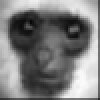
\includegraphics[width=0.2\textwidth]{result_13.jpg}}\hfill
	\subcaptionbox{Способ сохранения 10 в 5}{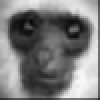
\includegraphics[width=0.2\textwidth]{result_ultra_mega_sposob_13.jpg}}
\end{figure}

\subsection{Большое изображение}
Из-за долгого времени работы алгоритма, на большом изображения такое маленькое разбиение не тестировалось.

\begin{figure}[h]
	\subcaptionbox{Фрактальное сжатие 6 в 3}{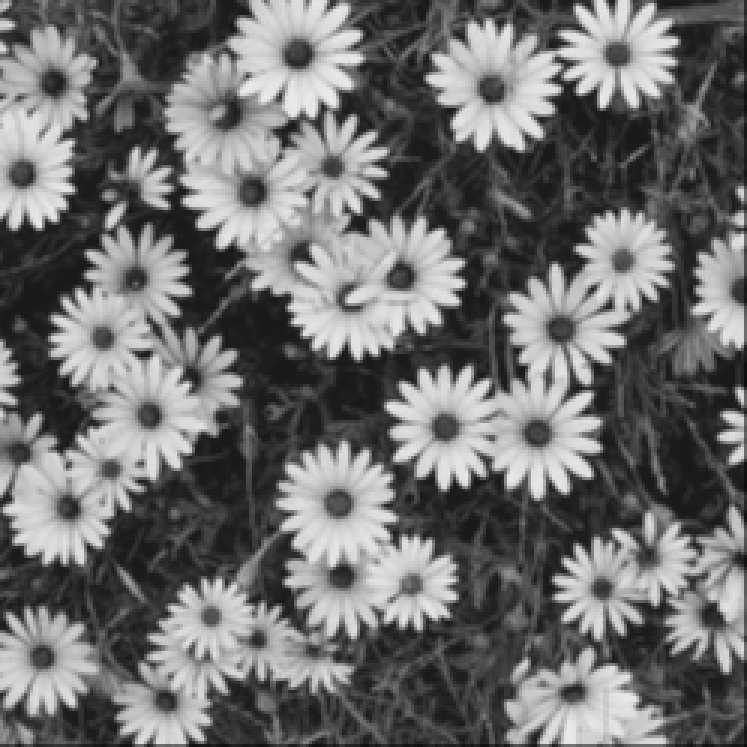
\includegraphics[width=0.2\textwidth]{result_2.jpg}}\hfill
	\subcaptionbox{Способ сохранения 6 в 3}{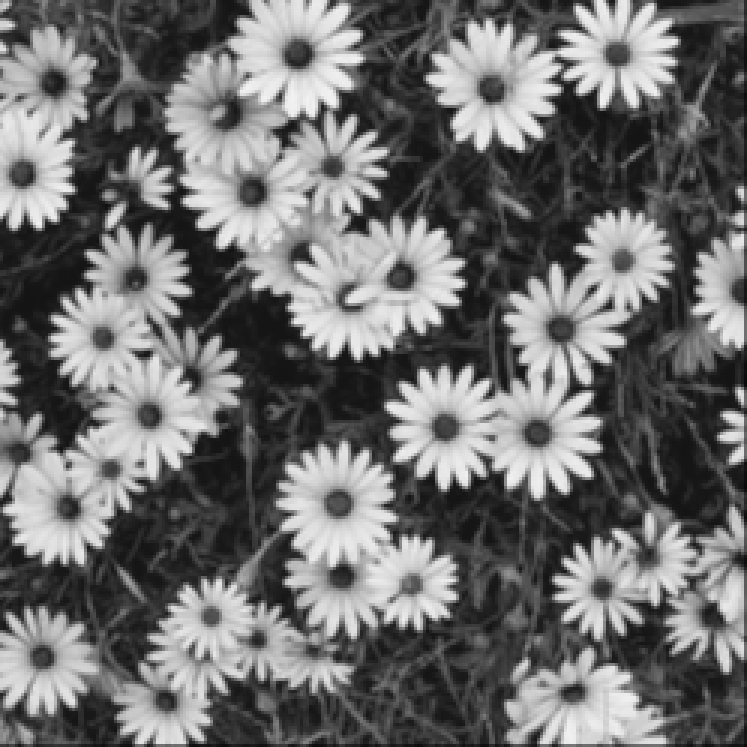
\includegraphics[width=0.2\textwidth]{result_ultra_mega_sposob_2.jpg}}\hfill
	\subcaptionbox{Фрактальное сжатие 8 в 4}{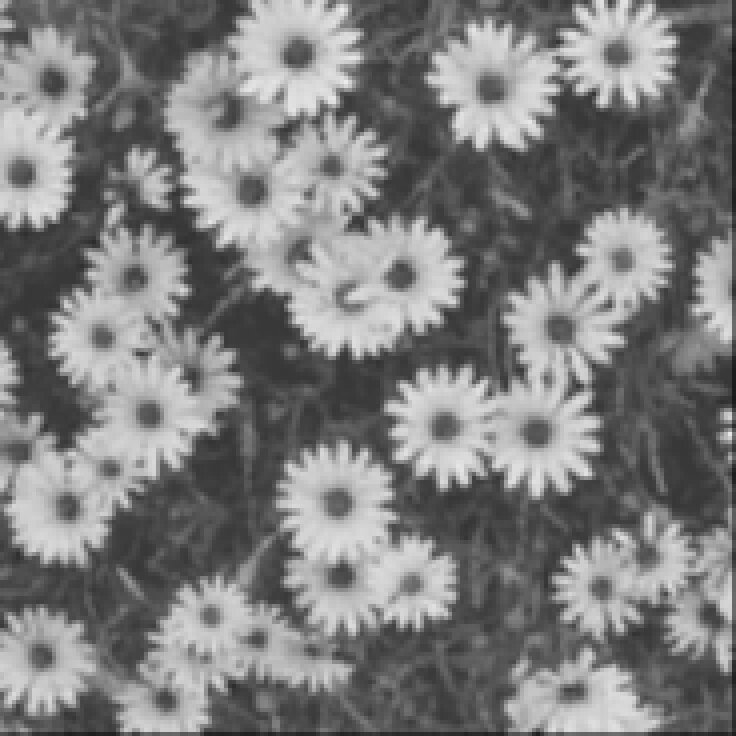
\includegraphics[width=0.2\textwidth]{result_22.jpg}}\hfill
	\subcaptionbox{Способ сохранения 8 в 4}{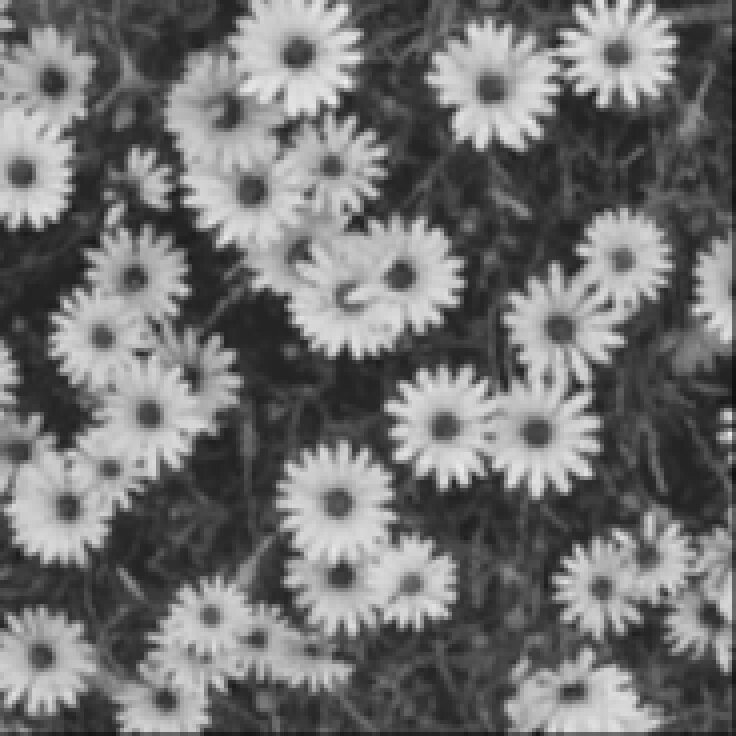
\includegraphics[width=0.2\textwidth]{result_ultra_mega_sposob_22.jpg}}
\end{figure}

\begin{figure}[h]
	\centering
	\subcaptionbox{Фрактальное сжатие 10 в 5}{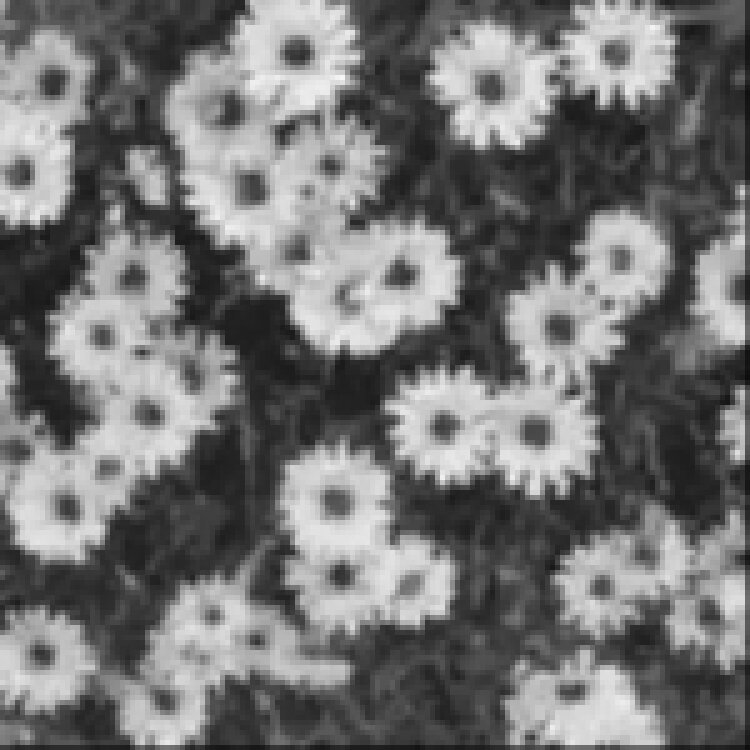
\includegraphics[width=0.2\textwidth]{result_23.jpg}}\hfill
	\subcaptionbox{Способ сохранения 10 в 5}{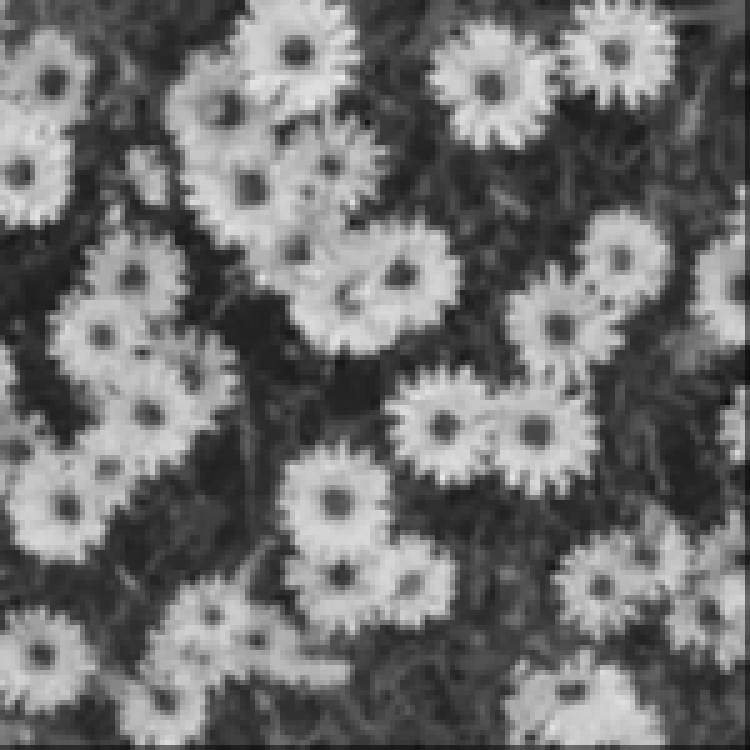
\includegraphics[width=0.2\textwidth]{result_ultra_mega_sposob_23.jpg}}
	\label{fig:mpr}
\end{figure}

\subsection{Опрос}

Для выявления лучших коэффициентов сжатия было опрошено 8 человек и получены следующие результаты:

Для маленького изображения:

\begin{figure}[h]
	\centering
	\subcaptionbox{Маленькое изображение}{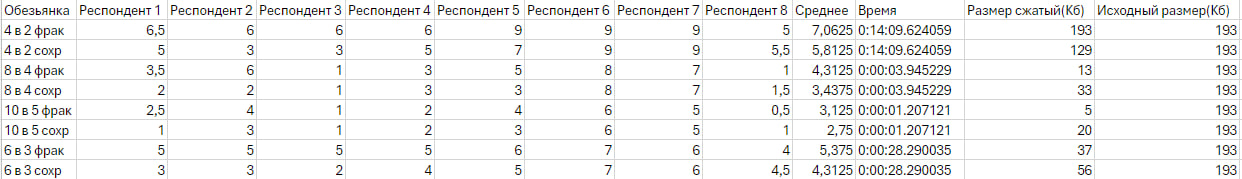
\includegraphics[width=1.3\textwidth]{opros_low.jpg}}\hfill
	\subcaptionbox{Большое изображение}{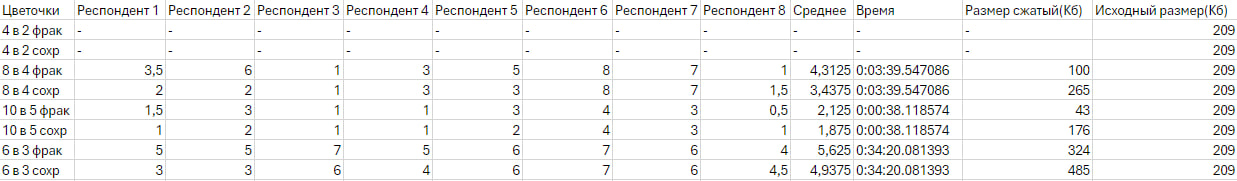
\includegraphics[width=1.3\textwidth]{opros_hi.jpg}}
\end{figure}

Из результатов опроса видно, что для малых изображений лучше всего использовать сжатие 6 в 3, т.к. оно не сильно затратно по времени и имеет хорошую четкость. Для больших изображений лучше использовать сжатие 8 в 4, хотя при таком сжатия существенно падает качество изображения, но время затраченное на это не столь велико. Именно такие коэффициенты сжатия будем считать оптимальными.

\section{Сжатие других изображений(цветных)}

\begin{figure}[h]
	\centering
	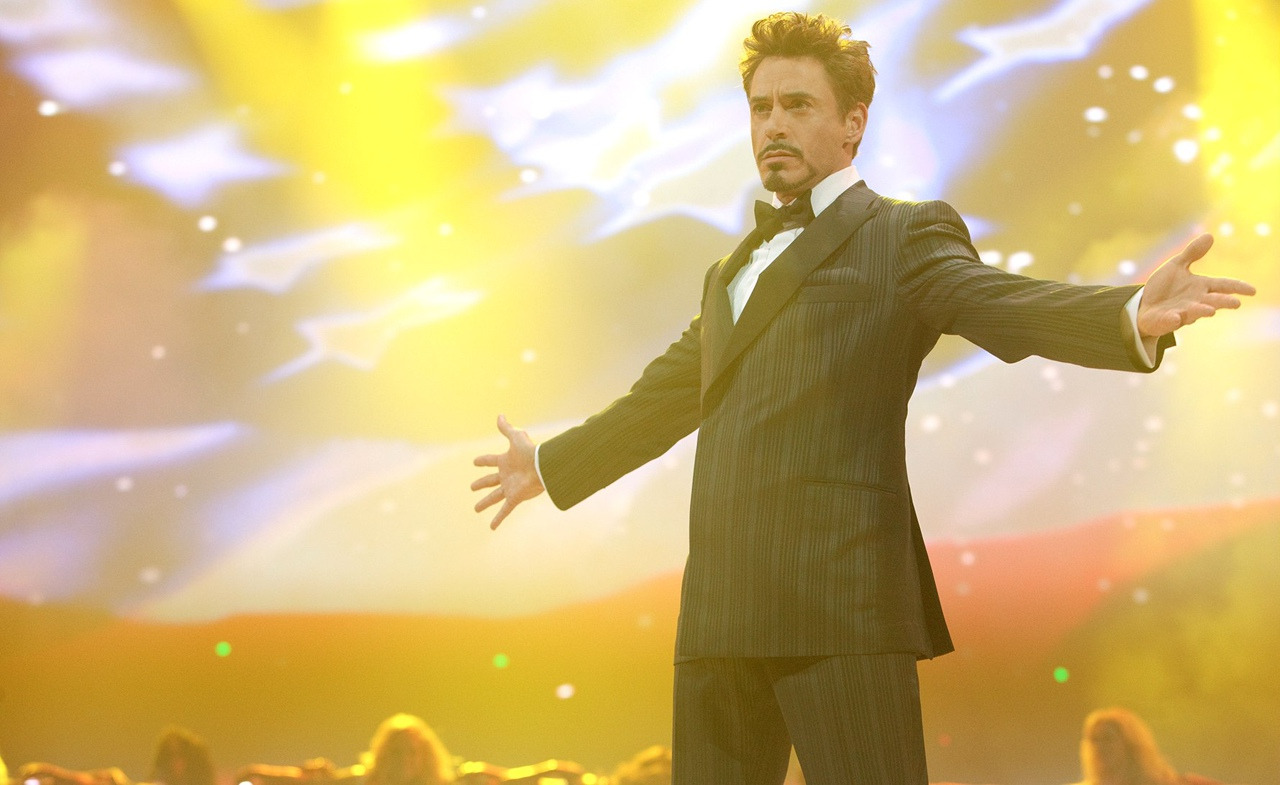
\includegraphics[width=0.4\linewidth]{input_3.jpg}
	\caption{Исходная картинка 3926 Кб}
	\label{fig:mpr}
\end{figure}

На данном изображении получились следующие результаты по времени(отсутствует результат 6 в 3 т.к. в программе выбор между максимальным сжатием/максимальным сохранением качества/оптимальное сжатие):
1. 10 в 5: 0:02:15.822430

2. 8 в 4: 0:12:21.176291

\begin{figure}[h]
	\subcaptionbox{Фрактальное сжатие 8 в 4}{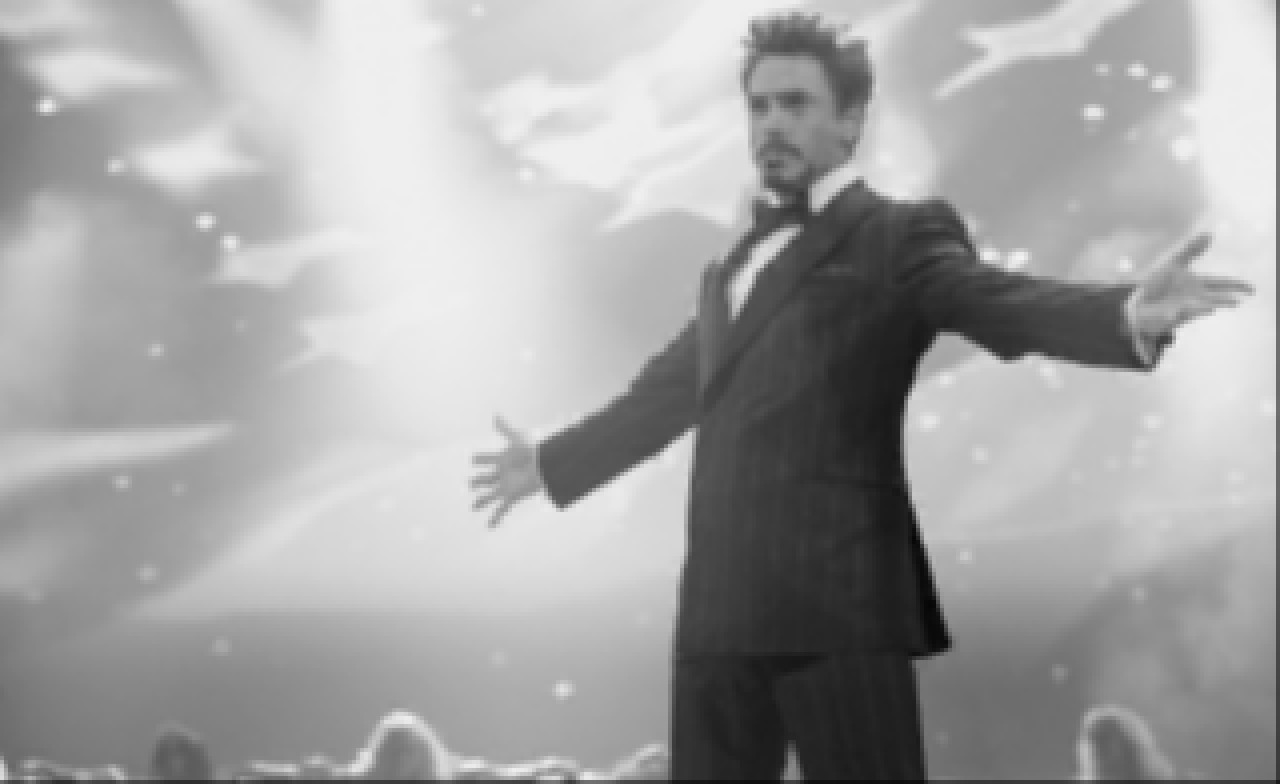
\includegraphics[width=0.2\textwidth]{result_31.jpg}}\hfill
	\subcaptionbox{Способ сохранения 8 в 4}{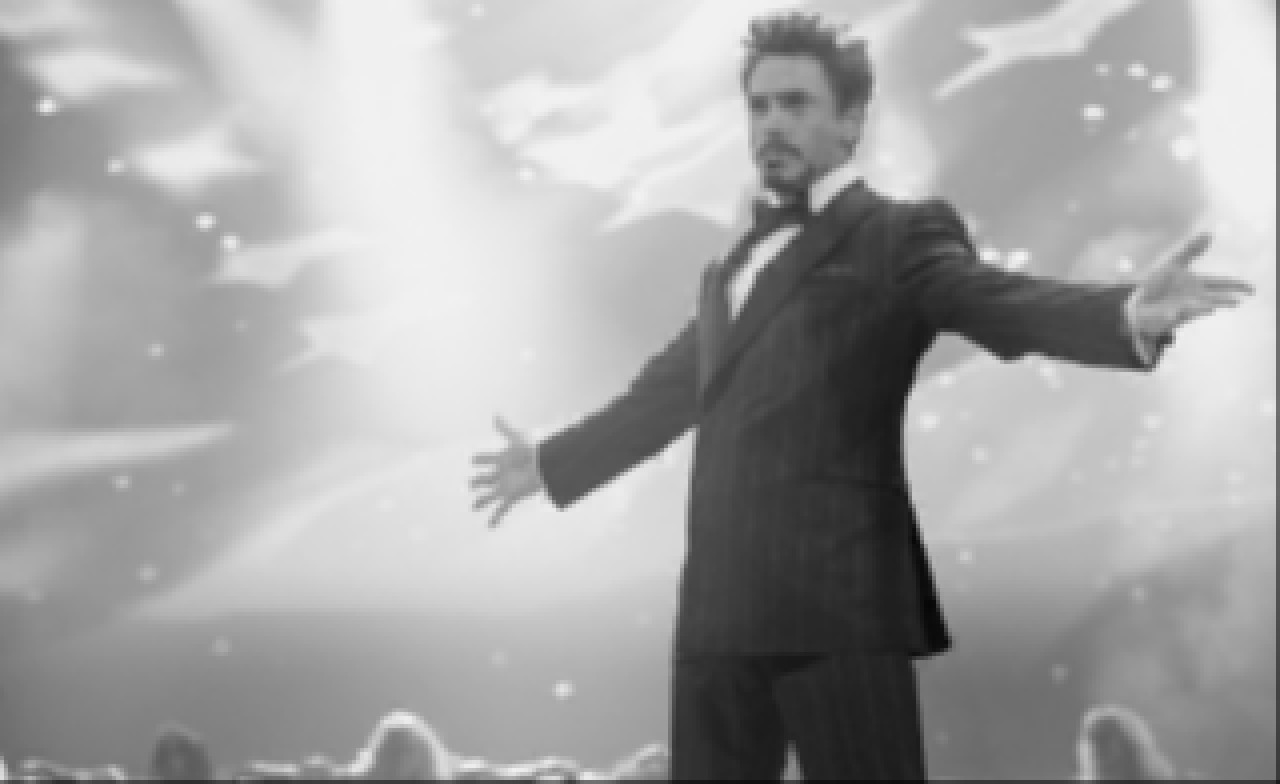
\includegraphics[width=0.2\textwidth]{result_ultra_mega_sposob_31.jpg}}\hfill
	\subcaptionbox{Фрактальное сжатие 10 в 5}{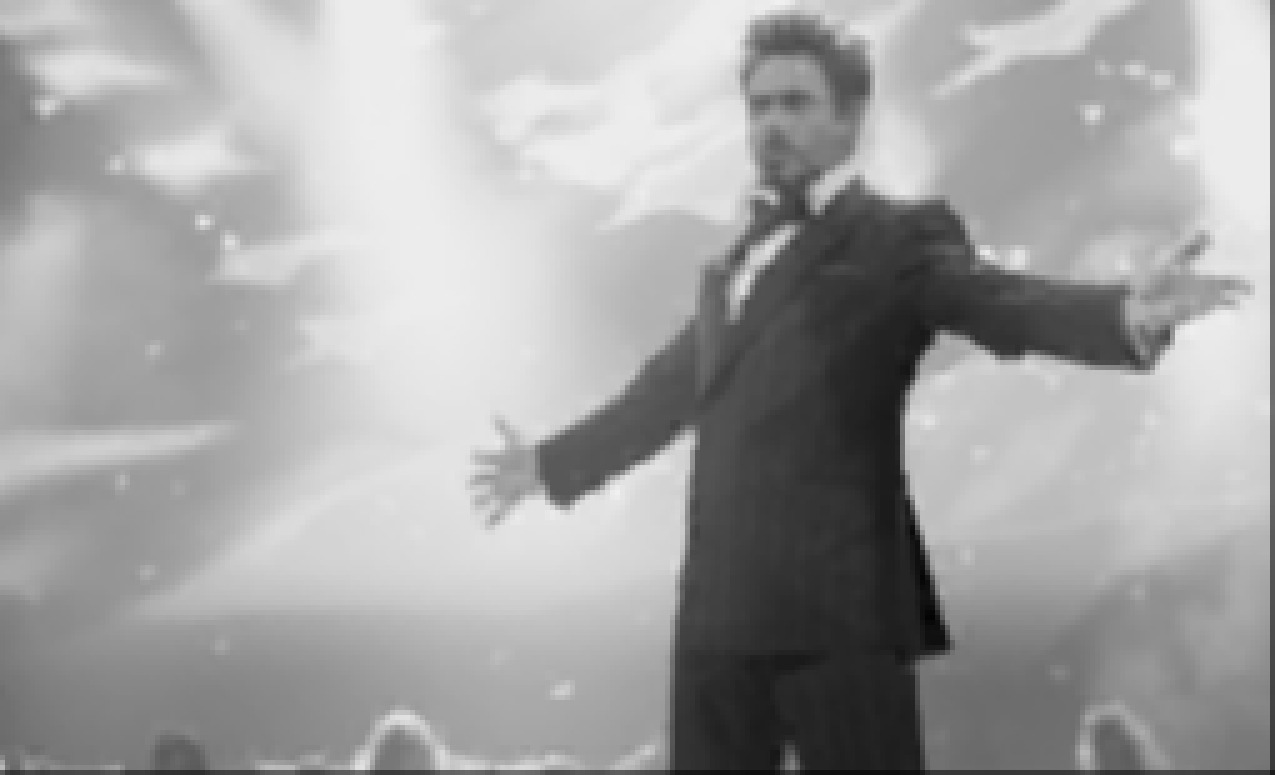
\includegraphics[width=0.2\textwidth]{result_33.jpg}}\hfill
	\subcaptionbox{Способ сохранения 10 в 5}{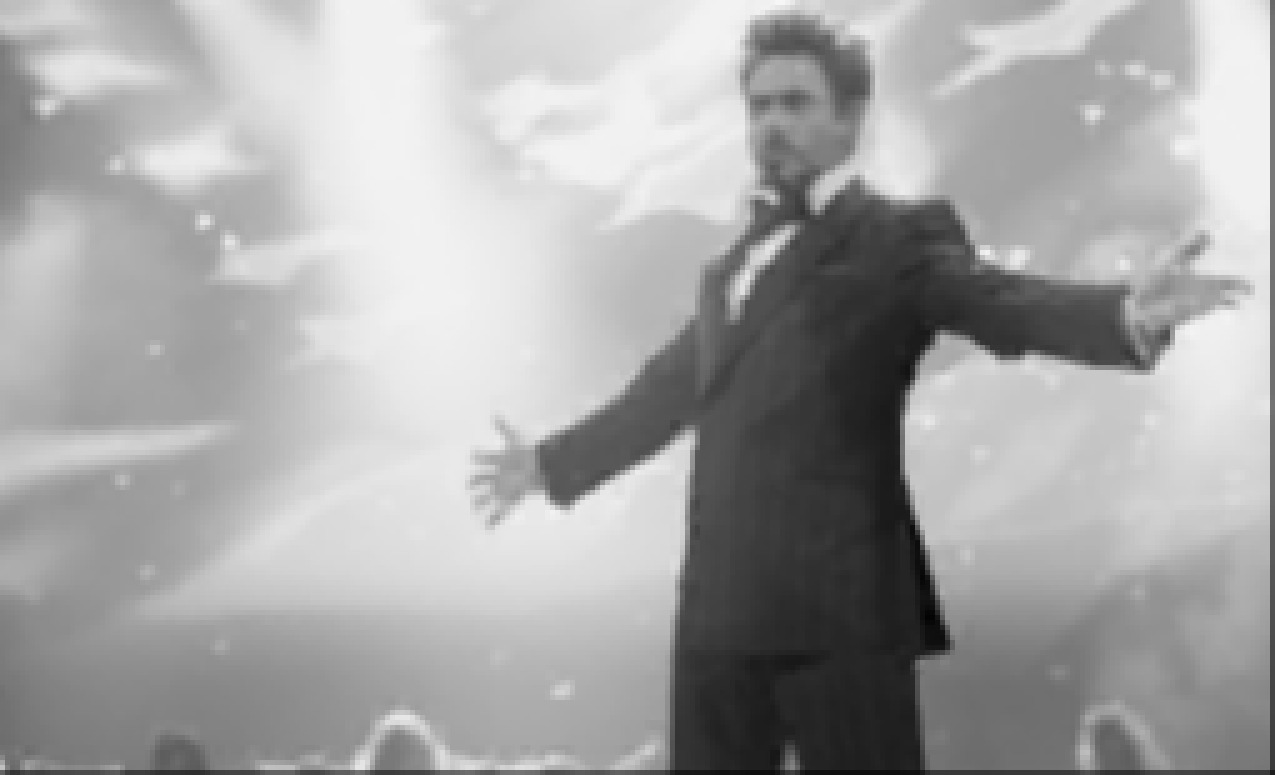
\includegraphics[width=0.2\textwidth]{result_ultra_mega_sposob_33.jpg}}
\end{figure}

  
\end{document}